\section{Stellwerkstechnik}\label{text:Grundlagen:Stellwerkstechnik}

Mit der Eröffnung der ersten Eisenbahnstrecke 1825 in England begann ein neues Zeitalter. Die Eisenbahn ermöglichte es, Personen und Güter schneller und effizienter zu transportieren als je zuvor. Mit zunehmendem Verkehr auf der Schiene stieg auch die Notwendigkeit der Sicherung der Fahrwege. Dieser Abschnitt behandelt die Grundlagen der Stellwerkstechnik, wie sie bei realen Eisenbahnen eingesetzt wird. Dabei wird zunächst der theoretische Hintergrund erläutert. Anschließend werden die drei geläufigsten technischen Umsetzungen vorgestellt. Diese sind mechanische, Relais- und elektronische Stellwerke. Zuletzt wird auf die neueste Entwicklung, das digitale Stellwerk, eingegangen.

\subsection{Grundlagen der Stellwerkstechnik}\label{text:Grundlagen:Stellwerkstechnik:Grundlagen-der-Stellwerkstechnik}

In den Anfangsjahren der Eisenbahn wurde die Notwendigkeit von Sicherungssystemen schnell deutlich. Ein großer Fortschritt war der Einsatz von Telegraphen, um Zugbewegungen zwischen Bahnhöfen zu koordinieren --- ein Verfahren, das heute noch unter dem Namen \textit{Zugleitbetrieb} angewandt wird. Jedoch war dieses Verfahren nicht ausreichend, um die Sicherheit der Fahrwege zu gewährleisten. So kam es immer wieder zu schweren Unfällen mit vielen Toten. Dies führte in der Folge zur Entwicklung elaborierter Sicherungssysteme, die letztlich in die heutige Stellwerkstechnik mündeten. In diesem Abschnitt werden die wichtigsten Konzepte der Stellwerks- und Sicherungstechnik erläutert.

\subsubsection*{Streckenblock}\label{text:Grundlagen:Stellwerkstechnik:Sicherung-des-Schienenverkehrs:Streckenblock}

Das mit Abstand wichtigste Konzept der Sicherungstechnik ist der Streckenblock. Hierbei handelt es sich zunächst um ein theoretisches Konstrukt, das später mit technischen Mitteln angewandt wird. Eine Zugstrecke wird in logische Abschnitte unterteilt, die \textit{Streckenblöcke} oder \textit{Blockabschnitte}. Hierbei gilt die wichtigste Regel der Sicherungstechnik: in einem Streckenblock darf sich immer nur ein Zug zur selben Zeit befinden.

\subsubsection*{Signale}\label{text:Grundlagen:Stellwerkstechnik:Sicherung-des-Schienenverkehrs:Signale}

Ein Signal ist ein technisches Mittel, um den Zugverkehr zu steuern. Konkret sichert es die Einfahrt in einen Streckenblock ab. Signale können in zwei wesentlichen Bauarten ausgeführt sein: als Formsignal und als Lichtsignal. Formsignale sind die ältere Bauart und werden heute nur noch selten eingesetzt. Sie bestehen aus einem Mast, an dem ein oder mehrere bewegliche Arme angebracht sind. Die Stellung der Arme gibt die Bedeutung des Signals an. Lichtsignale sind die heute übliche Bauart. Sie bestehen aus einem Mast, an dem mehrere Lichter angebracht sind. Die Bedeutung des Signals wird durch die Anordnung und Farbe der Lichter angezeigt. In \autoref{abb:Grundlagen:Stellwerkstechnik:Signale} sind beispielhaft ein Form- und ein Lichtsignal dargestellt.

% https://de.wikipedia.org/wiki/Datei:Ks_Signal_NALB.jpg
% https://de.wikipedia.org/wiki/Datei:Formsignale.jpg
\begin{figure}[H]
    \centering
    \subfloat[\centering Formsignale]{{
        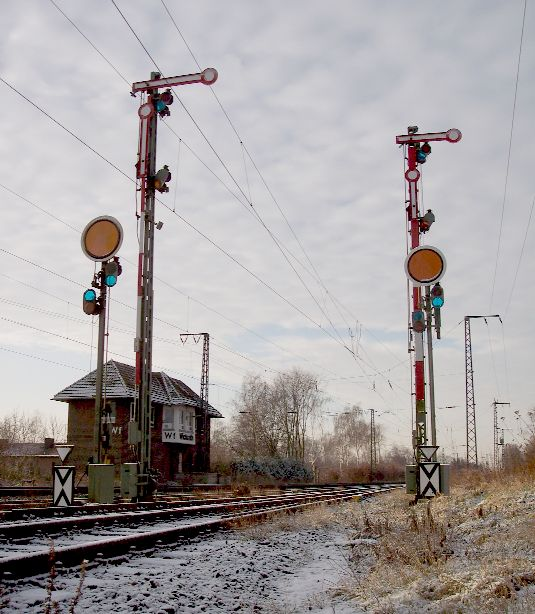
\includegraphics[width=.4\textwidth]{Assets/Images/2-Grundlagen/Formsignale.jpg}
    }}
    \qquad
    \subfloat[\centering Lichtsignal]{{
        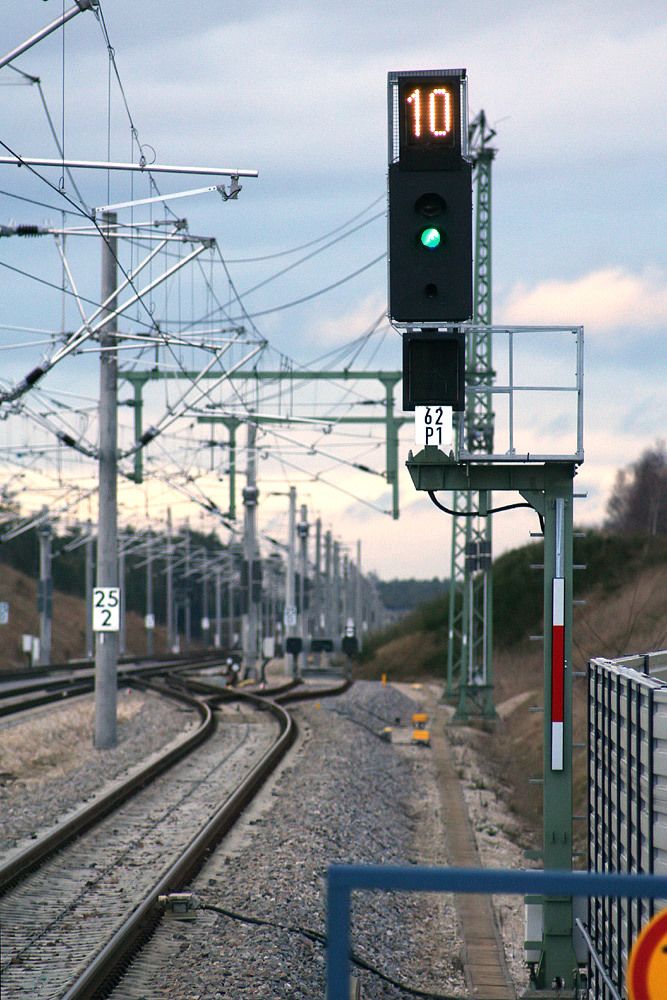
\includegraphics[width=.4\textwidth]{Assets/Images/2-Grundlagen/Ks-Signal.jpg}
    }}
    \caption{Beispiele für deutsche Eisenbahnsignale}\label{abb:Grundlagen:Stellwerkstechnik:Signale}
\end{figure}

In Deutschland sind mehrere Signalsysteme im Einsatz. Ein Signalsystem beschreibt die Bedeutung der Signale und die zugehörigen Signalbilder. Wie Ampeln im Straßenverkehr können Eisenbahnsignale einem Zug die Weiterfahrt erlauben oder verwehren. Außerdem können zulässige Höchstgeschwindigkeiten und die Richtung, in die ein Fahrweg eingestellt ist, angezeigt werden. Da diese Arbeit ihren Fokus nicht auf Signalisierung legt, soll auf dieses Thema nicht weiter eingegangen werden.

\subsubsection*{Weichen}\label{text:Grundlagen:Stellwerkstechnik:Sicherung-des-Schienenverkehrs:Weichen}

Eine Weiche ist ein technisches Mittel, um die Fahrtrichtung eines Zuges zu ändern. Sie besteht aus mehreren Schienen, die beweglich miteinander verbunden sind. Weichen gehören mit zu den wichtigsten Fahrwegelementen, da erst durch sie ein sinnvoller Eisenbahnbetrieb möglich wird. In \autoref{abb:Grundlagen:Stellwerkstechnik:Weichen} ist beispielhaft eine Weiche dargestellt.

% https://de.wikipedia.org/wiki/Datei:Handweiche_Bayreuth_Sankt_Georgen.JPG
\begin{figure}[H]
    \centering
    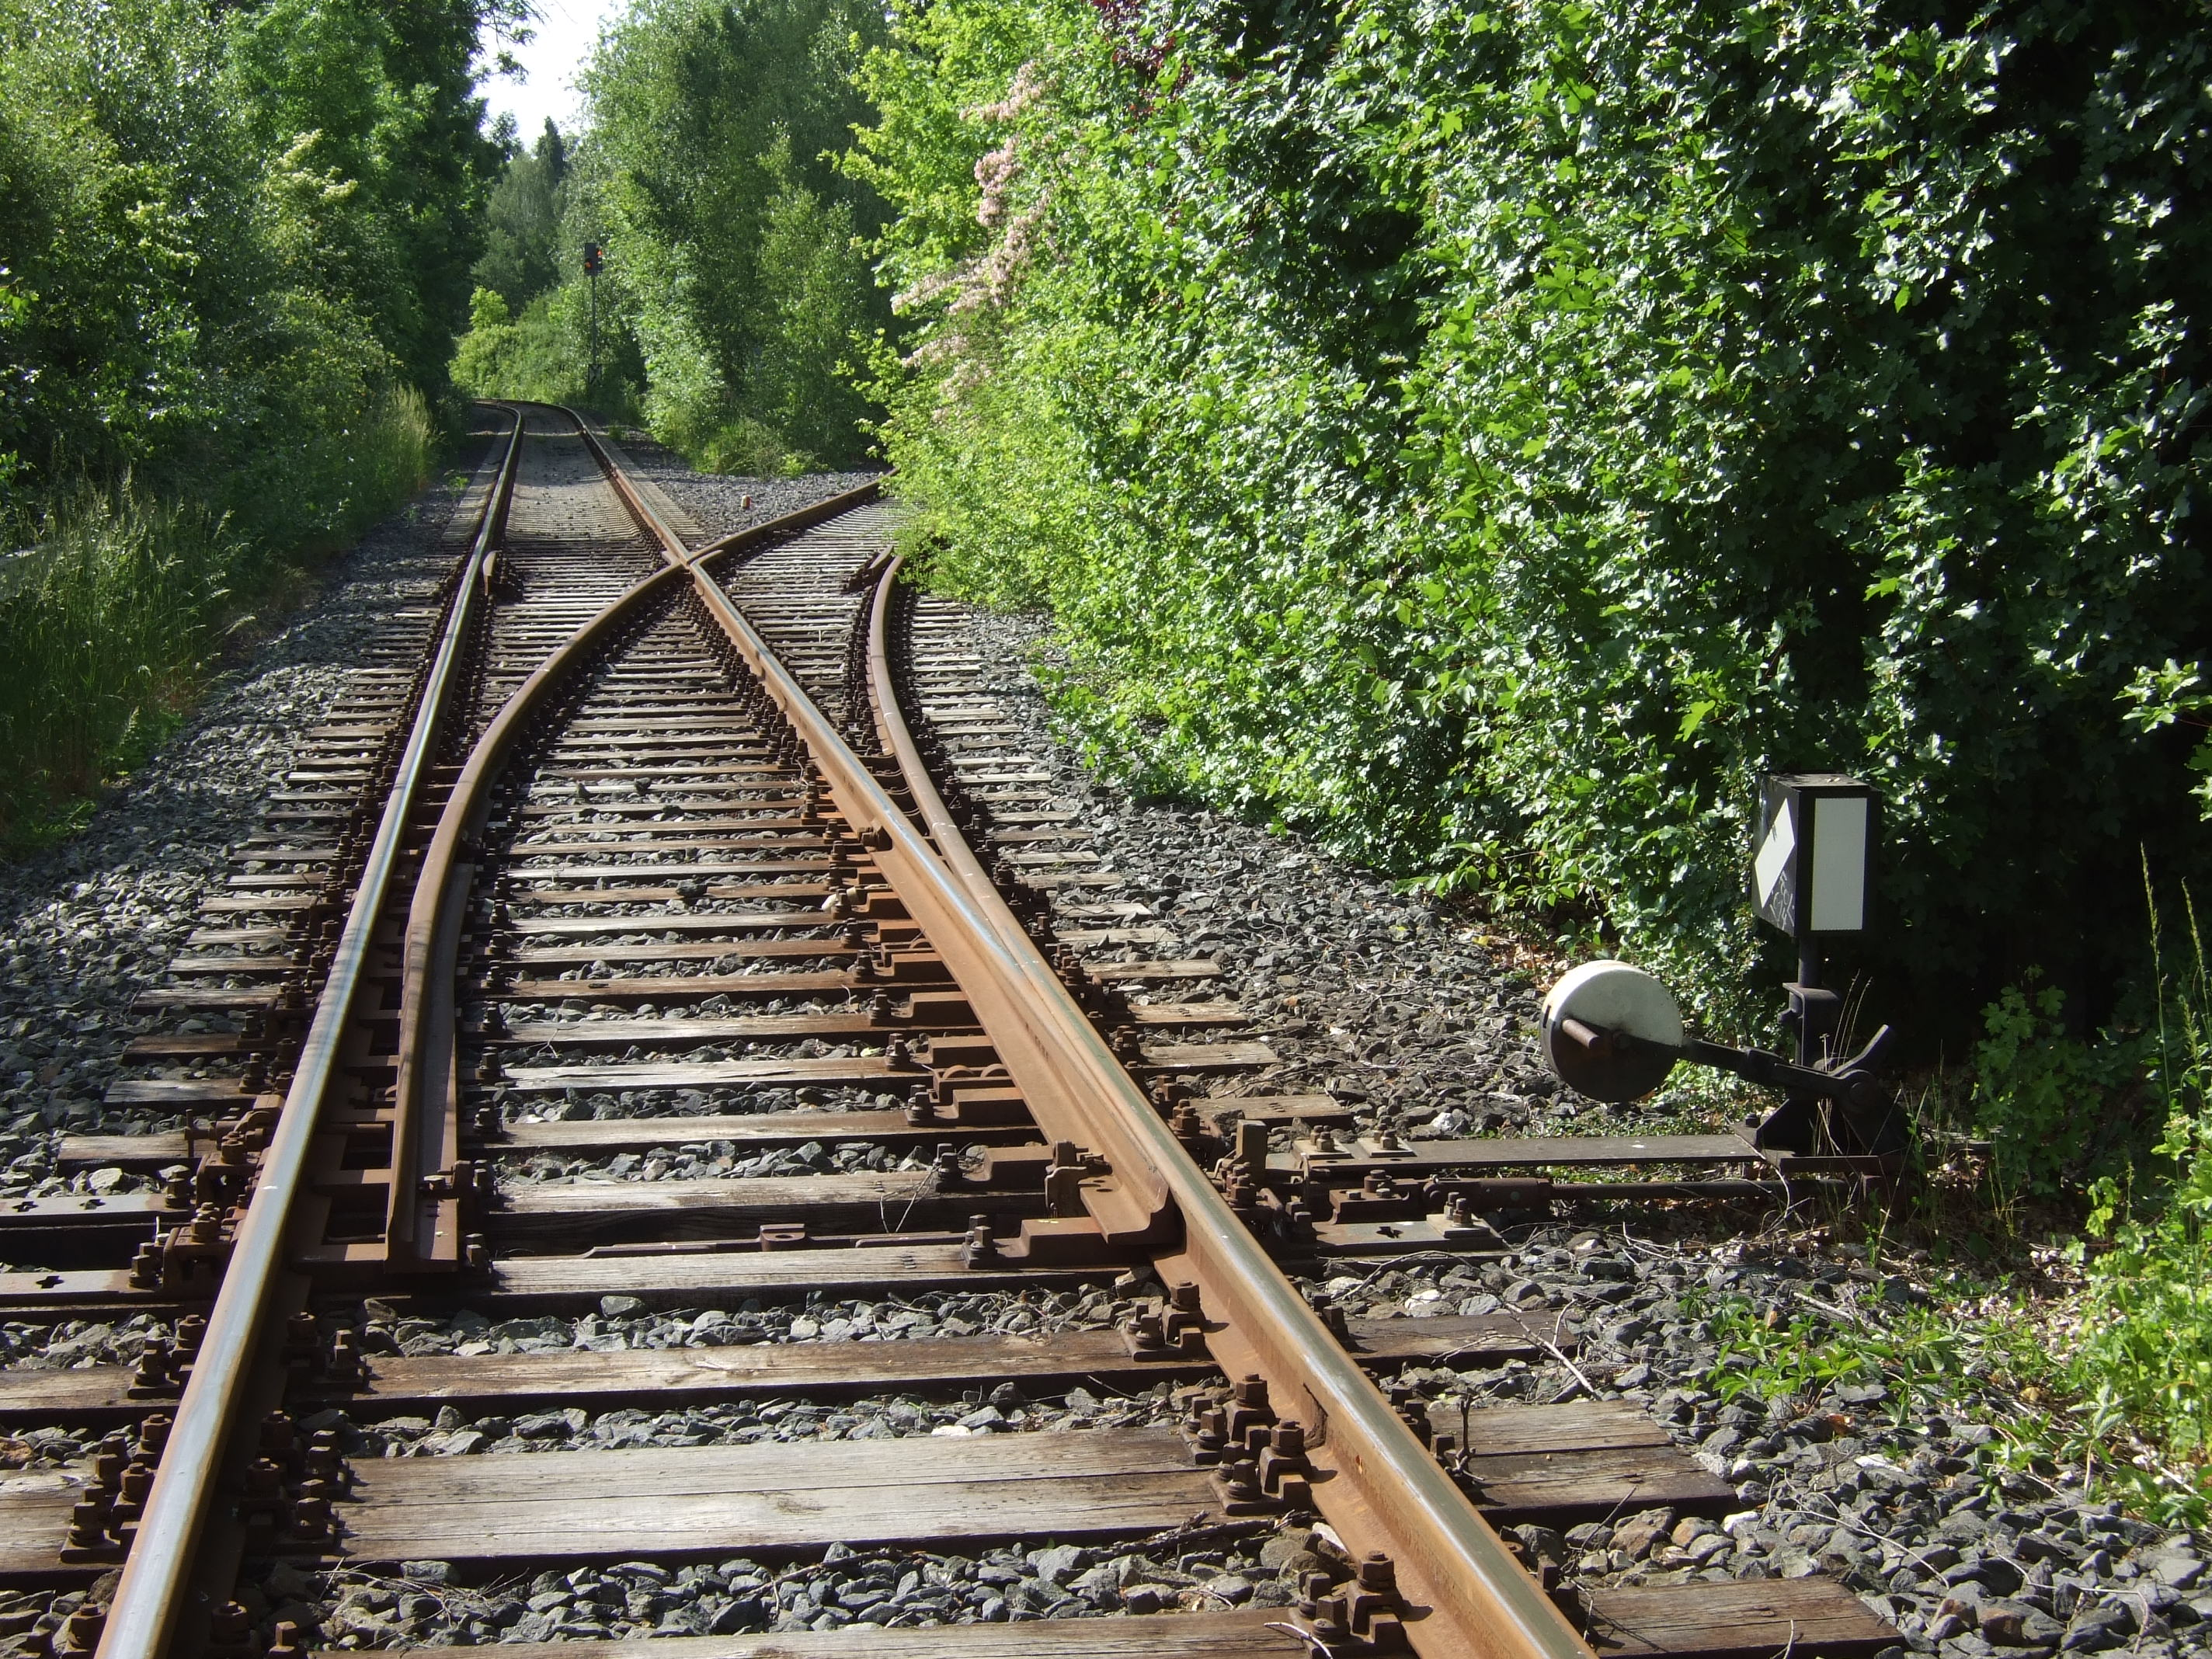
\includegraphics[width=.6\textwidth]{Assets/Images/2-Grundlagen/Handweiche.jpg}
    \caption{Beispiel für eine Weiche}\label{abb:Grundlagen:Stellwerkstechnik:Weichen}
\end{figure}

Weiche gibt es in vielen verschiedenen Ausführungen. Die wichtigste Unterscheidung ist die zwischen \textit{Handweichen} und \textit{elektrischen Weichen}. Handweichen werden von Hand umgestellt. Sie sind die ältere Bauart und werden heute nur noch selten eingesetzt. Elektrische Weichen werden von einem Stellwerk aus umgestellt und sind die heute übliche Bauart. Detaillierter Aufbau und Funktion einer Weiche sind für diese Arbeit nicht relevant. Dennoch soll dieses Thema der Vollständigkeit halber erwähnt werden, da das Konzept der Weiche im weiteren Verlauf dieser Arbeit wieder aufgegriffen wird.

\subsubsection*{Flankenschutz}\label{text:Grundlagen:Stellwerkstechnik:Sicherung-des-Schienenverkehrs:Flankenschutz}

Ein weiteres wichtiges Konzept der Sicherungstechnik ist der Flankenschutz. Er verhindert, dass ein Zug mit einem anderen Zug seitlich kollidiert, also in dessen Flanke fährt. Dies kann insbesondere dann auftreten, falls ein Zug eine ungeplante Fahr- oder Rollbewegung durchführt. Ein Beispiel hierfür ist das zu späte Bremsen bei der Einfahrt in einen Bahnhof. Um Flankenschutz zu gewährleisten, werden Weichen, die gar nicht von einem Zug befahren werden, so gestellt, dass ein auf einem anderen Gleis ungeplant fahrender Zug, nicht in die Flanke des anderen Zuges fahren kann. Um dieses Konzept zu verdeutlichen, sei in \autoref{abb:Grundlagen:Stellwerkstechnik:Flankenschutz} ein beispielhafter, vereinfachter Gleisplan dargestellt.

\todo{Besseres Bild für Flankenschutz finden (selber malen)}
\begin{figure}[H]
    \centering
    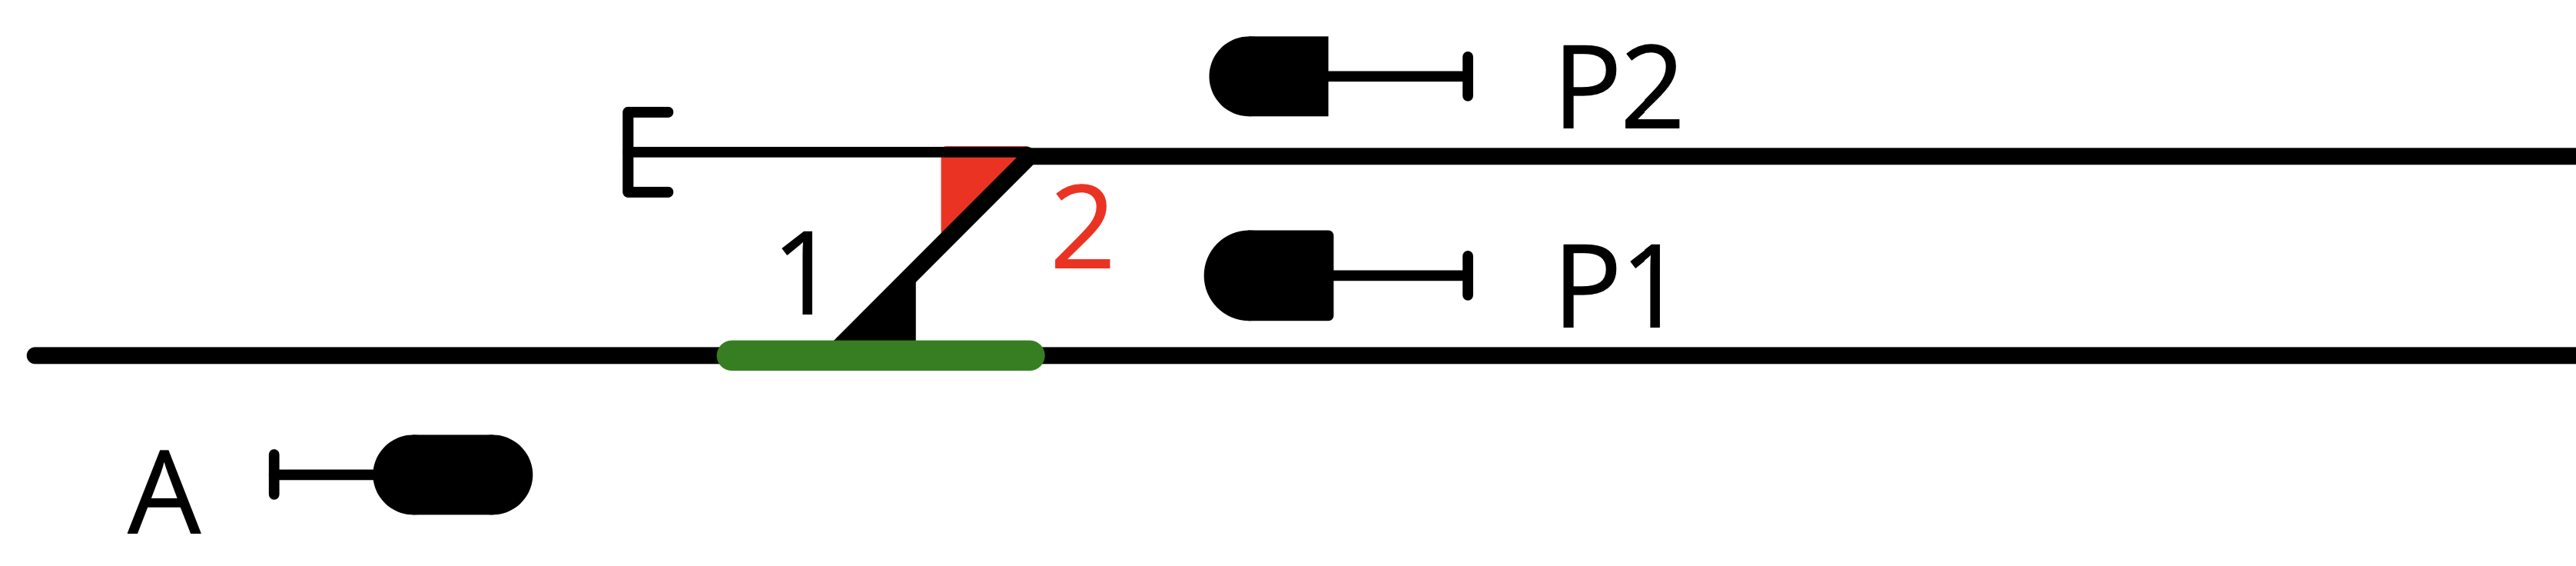
\includegraphics[width=\textwidth]{Assets/Images/2-Grundlagen/Flankenschutz.png}
    \caption{Beispiel für Flankenschutz}\label{abb:Grundlagen:Stellwerkstechnik:Flankenschutz}
\end{figure}

Sei folgendes Szenario gegeben: Es handelt sich um einen Bahnhof mit einem leichten Gefälle nach links. Weiche 2 hat scheinbar keinen Nutzen. Ein Zug steht vor Signal P2. Ein anderer fährt von Signal A nach N1 in den Bahnhof ein. Weiche 1 ist somit in Rechtslage. Jetzt kommt es beim Zug an P2 zu einer ungewollten Lösung der Bremsen und der Zug beginnt zu rollen. Würde Weiche 2 nicht existieren, käme es zu einer Kollision der beiden Züge. Durch Weiche 2 wird der rollende Zug jedoch in ein Stumpfgleis geleitet, wo er zum Stehen kommt. Es kommt zu keiner Kollision. Weiche 2 wird als \textit{Flankenschutzweiche} bezeichnet und hat in diesem einfachen Beispiel auch nur diese eine Funktion. Das Stellwerk stellt sicher, dass der Flankenschutz beim Stellen einer Fahrstraße immer gegeben ist. In der Praxis sind die Gleisanlagen jedoch meist weit umfangreicher und reine Flankenschutzweichen sind selten. Vielmehr sind Flankenschutzweichen Teil von Fahrwegen anderer Züge und nicht immer direkt zu erkennen.

Neben Weichen können auch Signale und andere Fahrwegelemente Flankenschutz bieten. Für diese Arbeit ist jedoch das Verständnis über Flankenschutzweichen ausreichend.

\subsubsection*{Fahrstraße}\label{text:Grundlagen:Stellwerkstechnik:Sicherung-des-Schienenverkehrs:Fahrstrasse}

Der Weg, den ein Zug zurücklegt, setzt sich aus verschiedenen Elementen zusammen:

\begin{itemize}
    \item Gleisabschnitte,
    \item Weichen,
    \item Signale,
    \item weitere Elemente, die hier nicht weiter relevant sind.
\end{itemize}

Die Kombination dieser Elemente wird als \textit{Fahrstraße} bezeichnet. Eine Fahrstraße beginnt und endet in der Regel an einem Signal. Der \ac{Fdl} fordert das Stellwerk zum stellen einer bestimmten Fahrstraße auf, indem er das Start- und Zielsignal eingibt. Aufgabe des Stellwerks ist es nun, einen Fahrweg zwischen den gewünschten Signalen zu finden. Hierbei müssen alle nötigen Fahrwegelemente gefunden und (im Falle von Weichen und Signalen) in die entsprechende Stellung gebracht werden. Wichtig ist hierbei auch das Gewähren von Flankenschutz. Beim Befahren einer Fahrstraße durch einen Zug, werden die Fahrwegelemente nach und nach frei gefahren und können vom Stellwerk wieder für andere Fahrstraßen verwendet werden. Man sagt, die Fahrstraße wird \textit{aufgelöst}.

\subsection{Mechanische Stellwerke}\label{text:Grundlagen:Stellwerkstechnik:Mechanische-Stellwerke}

\subsection{Relaisstellwerke}\label{text:Grundlagen:Stellwerkstechnik:Relaisstellwerke}

\subsection{Elektronische Stellwerke}\label{text:Grundlagen:Stellwerkstechnik:Elektronische-Stellwerke}

\subsection{Digitale Stellwerke}\label{text:Grundlagen:Stellwerkstechnik:Digitale-Stellwerke}
